\documentclass{beamer}


\setbeamerfont{footnote}{size=\tiny}
%\AtBeginSection[]
%{
%  \begin{frame}<beamer>
%%    \frametitle{Outline for Section \thesection}
%    \frametitle{Outline}
%    \tableofcontents[currentsection]
%  \end{frame}
%}

\newcommand{\OutlineRedux}
{
  \begin{frame}<beamer>
%    \frametitle{Outline for Section \thesection}
    \frametitle{Outline}
    \tableofcontents[currentsection]
  \end{frame}
}


\usepackage{algpseudocodex}
\usepackage{tikz}
\usetikzlibrary{positioning, arrows.meta}

\usetheme{CambridgeUS}
\setbeamercolor{title}{bg=red!65!black,fg=white}

\setbeamertemplate{sidebar right}
{
  \vfill%
  \llap{\insertlogo\hskip0.1cm}%
  \vskip2pt%
  \llap{\href{http://domdisanto.github.io}{Downloadable Slides}\hskip0.2cm}% NEW
  \vskip3pt% NEW
  \llap{\usebeamertemplate***{navigation symbols}\hskip0.1cm}%
  \vskip2pt%
}



% Bibliography Options 
\usepackage[url=false, doi=false, maxcitenames=1, isbn=false]{biblatex}
\addbibresource{GNN_Presentation.bib}

\title{Graphical Neural Networks}
%\subtitle{}
\author{Dominic DiSanto}
\institute[]{Department of Biostatistics, Harvard University}
\date{\today}


% Custom commands 
\newcommand{\nhood}{\mathcal{N}}
\newcommand{\Graph}{\mathcal{G}}
\newcommand{\NodeSet}{V}
\newcommand{\EdgeSet}{E}
\newcommand{\node}{v}
\newcommand{\nrepresent}{h}
\newcommand{\edge}{e}
\newcommand{\iter}{\kappa}
\newcommand{\Iter}{K}
\newcommand{\AdjMat}{\mathbf{A}}
\newcommand{\LapMat}{\mathbf{L}}

%%%%%%%%%%%%%%%%%%%%%%%%
    % START %%%%%%%%%%%%
%%%%%%%%%%%%%%%%%%%%%%%%
\begin{document}

\begin{frame}{Notes (To Be Deleted)}
    \begin{itemize}
        \item Nvidia article has some refs to earliest uses/applications of GNNs at \url{https://blogs.nvidia.com/blog/what-are-graph-neural-networks/}; \url{https://ieeexplore.ieee.org/document/4700287} First in 2009, really first application in 2016 \url{https://arxiv.org/abs/1609.02907}
        \item Pinterest in 2017 published GraphSage \url{https://arxiv.org/abs/1706.02216}
    \end{itemize}
\end{frame}


\begin{frame}{Other application placeholder}
    \begin{itemize}
        \item ETA analysis for travel, 2021 \url{https://arxiv.org/pdf/2108.11482.pdf}
    \end{itemize}
\end{frame}


\begin{frame}
\maketitle
\end{frame}

\begin{frame}{Outline}
\tableofcontents 
\end{frame}


\section{Set-Up and Motivation \textcolor{red}{5ish minutes}}

\begin{frame}{Goals}
    \begin{itemize}\setlength\itemsep{8mm}
        \item Provide a useful overview of Graphical Neural Networks (GNN)
        \begin{itemize}
            \item Motivation for necessity of GNN's 
            \item Provide a general framework of fitting 
        \end{itemize}
        \item Describe applications and extensions of the general GNN model 
        \begin{itemize}
            \item \textcolor{red}{List specific instances here}
        \end{itemize}
    \end{itemize}
\end{frame}


\begin{frame}{KG Application}
    \textcolor{red}{Image here}
\end{frame}

\begin{frame}{Multi-modal Biomedical Data}
    \begin{figure}
        \centering 
        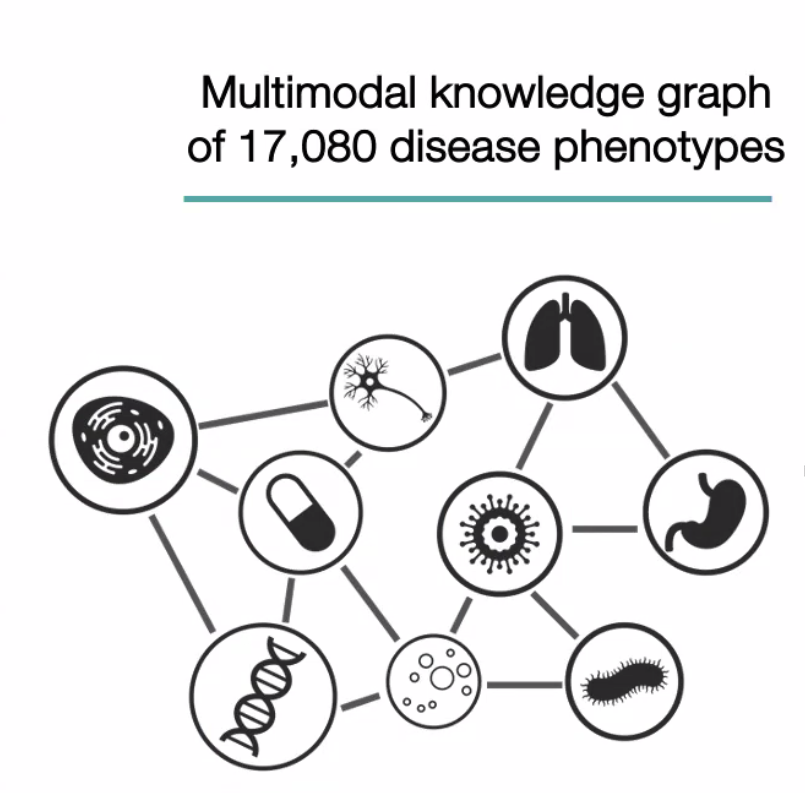
\includegraphics[scale=0.2]{MultimodalPreview.png}
    \end{figure}
    Image courtesy of partial figure from McDermott et al. {\it Structure-inducing pre-training} \cite{mcdermott_structure-inducing_2023}
\end{frame}


\begin{frame}{Molecular/Biochemical}
    \begin{figure}
        \centering
        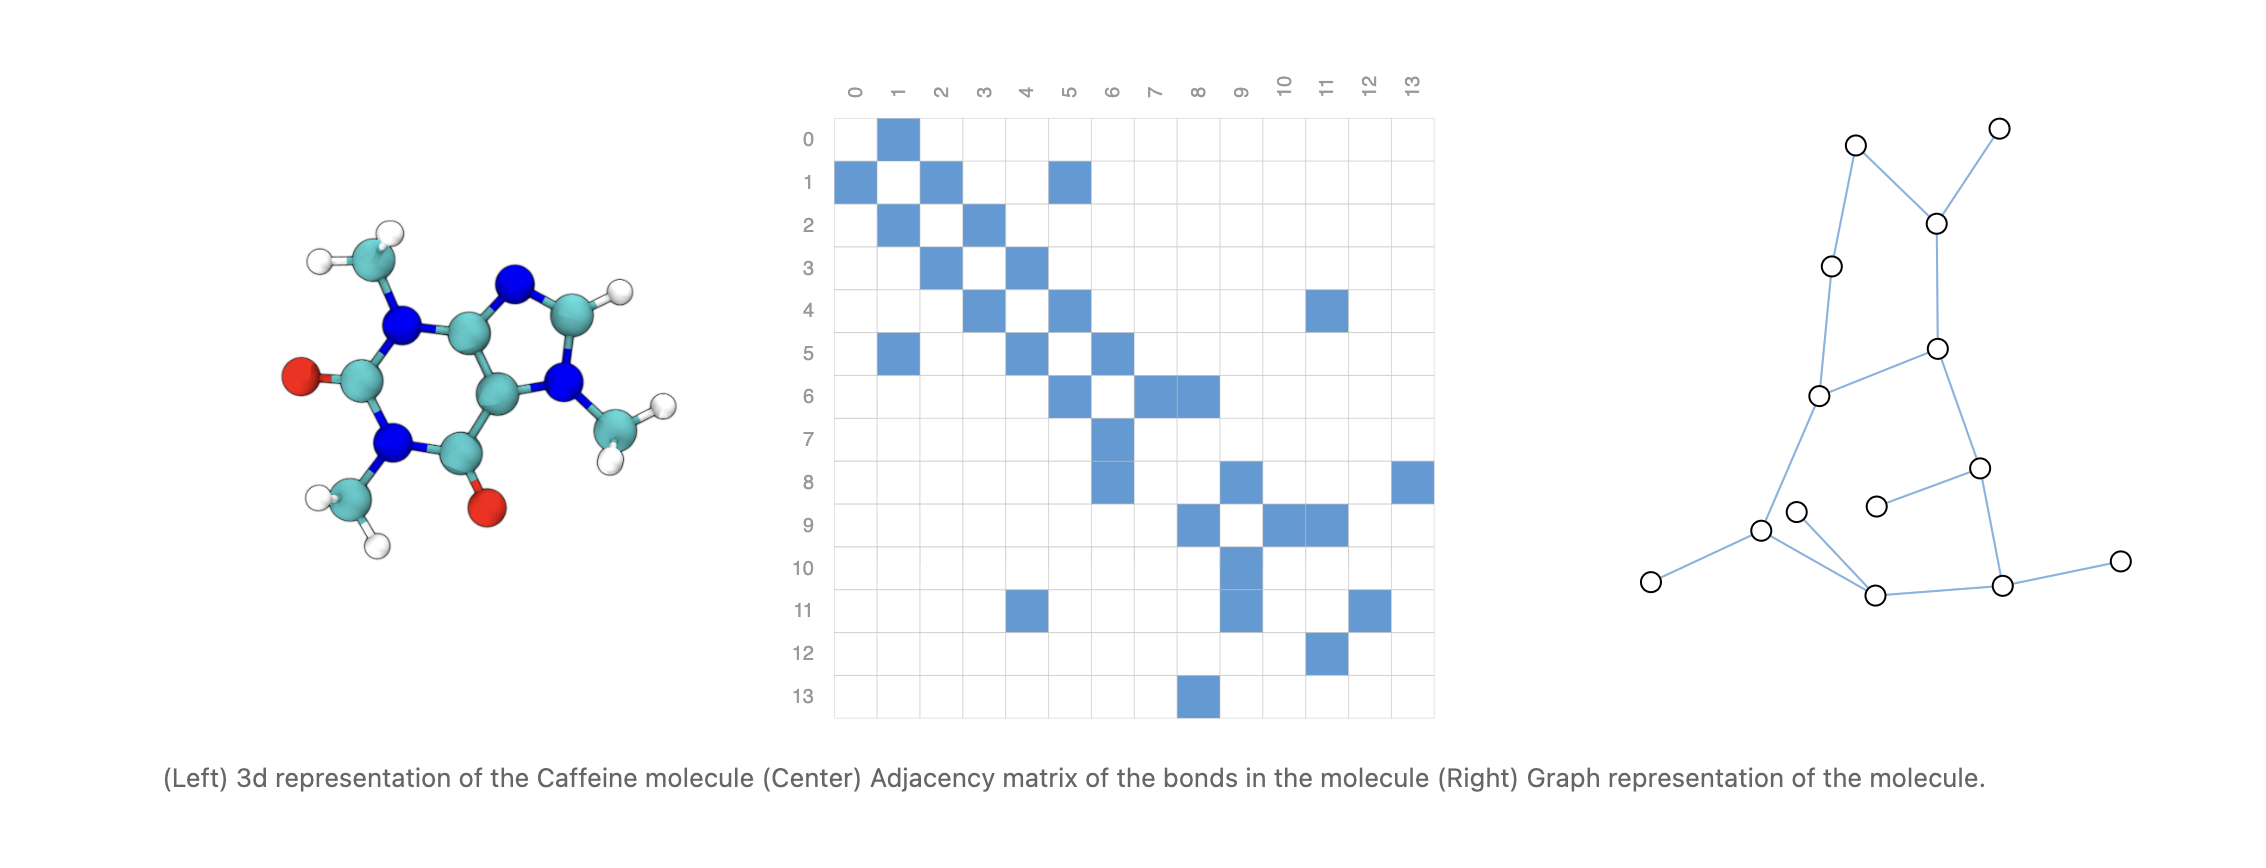
\includegraphics[scale=0.3]{Caffeine_Graph.png}
    \end{figure}
    Image courtesy of \url{https://distill.pub/2021/gnn-intro/} \cite{sanchez-lengeling_gentle_2021}
\end{frame}

\begin{frame}{Protein Folding \textcolor{red}{Maybe drop? 4 examples probably unnecessary}}
    \textcolor{red}{Image/example here }
\end{frame}

\begin{frame}{Motivation}
    \begin{itemize}
        \item Want to utilize the input structure of the graph
        \begin{itemize}
            \item Respect/Maintain
            \item Update/Estimate
        \end{itemize} 
        \item \color{red} Why do "regular" NN's/CNN's fail on graphical data? 2009 paper offers pre-GNN data processing led to information loss 
        \item Permutation invariance/Permutation invariant hypotheses 
    \end{itemize}
\end{frame}



\begin{frame}{Notation/Set-Up}
    \begin{columns}[T] % align columns at the top
        \begin{column}{.7\textwidth}
            \begin{itemize}%{.5\textwidth}
                \setlength\itemsep{8mm}
%                \item Consider random vector $X \sim F(\boldsymbol\mu, \Sigma)$ and precision matrix $\Theta \equiv \Sigma^{-1}$
                \item Consider the graph $\Graph = (\NodeSet, \EdgeSet), \EdgeSet \subseteq \NodeSet \times \NodeSet$, where any node $\node$ has a related "feature vector" $x_\node \in \mathbb{R}^d$
                \item Let $\nhood_s(\node)$ represent the $s$-hop neighborhood of any node $\node$ (and implicitly $\nhood(\node) \equiv \nhood_1(\node)$)
                \item Can construct adjacency matrix $\AdjMat \in \mathbb{R}^{|\NodeSet| \times |\NodeSet|}$ describing edge set $\EdgeSet$ 
                \begin{itemize} 
                    \item $\AdjMat_{ij}=\mathbb{I}\{(i,j) \in \EdgeSet\}$ 
                    \item Adjacency "lists" often used for memory efficiency and permutation invariance
                \end{itemize}
            \end{itemize}
        \end{column}
        \begin{column}{.3\textwidth}
            %\begin{figure}
                \centering
            \scalebox{0.9}{
                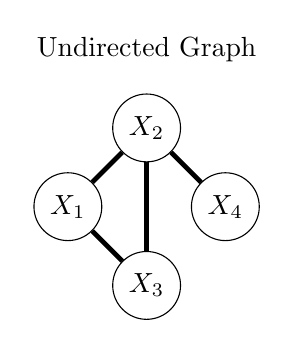
\begin{tikzpicture}
                \node[circle, draw] (A) at (0,0) {$X_1$};
                \node[circle, draw] (B) at (1,1) {$X_2$};
                \node[circle, draw] (C) at (1,-1) {$X_3$};
                \node[circle, draw] (D) at (2,0) {$X_4$};
                \node[] (capt) at (1, 2) {Undirected Graph};
                \draw[line width=0.6mm] (A) -- (B);
                \draw[line width=0.6mm] (A) -- (C);
                \draw[line width=0.6mm] (B) -- (D);
                \draw[line width=0.6mm] (C) -- (B);
            \end{tikzpicture}
            }
            %\caption{Undirected Graph}
            %\end{figure}
            \\ \vspace{3mm}
            \scalebox{0.9}{
            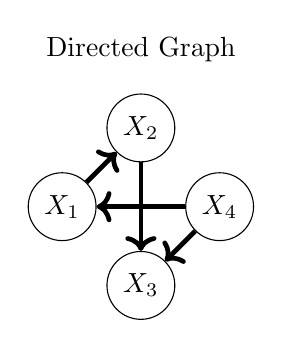
\begin{tikzpicture}%[opacity=0.2]
                \node[circle, draw] (A) at (0,0) {$X_1$};
                \node[circle, draw] (B) at (1,1) {$X_2$};
                \node[circle, draw] (C) at (1,-1) {$X_3$};
                \node[circle, draw] (D) at (2,0) {$X_4$};
                \node[] (capt) at (1, 2) {Directed Graph};
                \draw [line width=0.6mm, ->]
                    (A) edge (B)
                    (D) edge (A) 
                    (D) edge (C) 
                    (B) edge (C);
            \end{tikzpicture}
            }
        \end{column}
    \end{columns}
\end{frame}


\begin{frame}{Adjacency Representations}
\begin{itemize}\setlength\itemsep{8mm}
    \color{red}
    \item Adjacency matrix can be prohibitively large but likely sparse, is also permutable but DNN's are not permutation invariant, undesirable 
    \item Can store an adjacency list
    \item Can use Laplacian matrix $\LapMat = \text{diag}(\AdjMat\mathbf{1}_{|\NodeSet|}) - \AdjMat$
    \end{itemize}
\end{frame}



\section{General Construction \textcolor{red}{10-20ish minutes}}
\OutlineRedux 


\begin{frame}{What do we estimate about graph structure?}
    \textcolor{red}{See supp note 1 on Multimodal learning with graphs}
    \begin{gather*}
        \text{GNN's can be }
        \begin{cases}
            \text{Node-wise }\Phi(\Graph, x): (x\in \NodeSet) \rightarrow \mathbb{R}^m 
            \\  \\ 
            \text{Edge-wise }\Phi(\Graph, e): (e\in \EdgeSet) \rightarrow \mathbb{R}^m  
            % can predict edge weights and prune to determine "edge presence", but I believe that GNN's take edge sets as input and preserve these edgesets 
            \\ \\ 
            \text{Graph-level level }\Phi(\Graph) %\rightarrow \mathbb{R}^m 
            \end{cases}            
    \end{gather*}
\end{frame}

\begin{frame}{}
    An overly simple representation: \newline 
    \begin{columns}[T]
    \begin{column}{0.3\textwidth}
        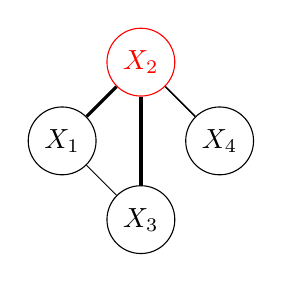
\begin{tikzpicture}
            \node[circle, draw] (A) at (0,0) {$X_1$};
            \node[circle, color=red, draw] (B) at (1,1) {$X_2$};
            \node[circle, draw] (C) at (1,-1) {$X_3$};
            \node[circle, draw] (D) at (2,0) {$X_4$};
            \draw[line width=0.4mm] (A) -- (B);
            \draw[line width=0.1mm] (A) -- (C);
            \draw[line width=0.2mm] (B) -- (D);
            \draw[line width=0.6mm] (C) -- (B);
        \end{tikzpicture}
    \end{column}
    \begin{column}{0.4\textwidth}
       % \begin{gather*}
            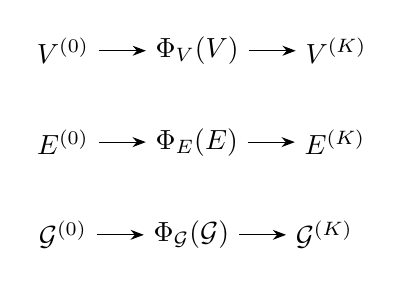
\begin{tikzpicture}[node distance=0.6cm,>=Stealth]
                % Nodes
                \node (NodeSet0) {$\NodeSet^{(0)}$};
                \node[right=of NodeSet0] (PhiNodeSet) {$\Phi_\NodeSet(\NodeSet)$};
                \node[right=of PhiNodeSet] (NodeSetIter) {$\NodeSet^{(\Iter)}$};
              
                \node[below=of NodeSet0] (EdgeSet0) {$\EdgeSet^{(0)}$};
                \node[right=of EdgeSet0] (PhiEdgeSet) {$\Phi_\EdgeSet(\EdgeSet)$};
                \node[right=of PhiEdgeSet] (EdgeSetIter) {$\EdgeSet^{(\Iter)}$};
              
                \node[below=of EdgeSet0] (Graph0) {$\Graph^{(0)}$};
                \node[right=of Graph0] (PhiGraph) {$\Phi_\Graph(\Graph)$};
                \node[right=of PhiGraph] (GraphIter) {$\Graph^{(\Iter)}$};
              
                % Arrows
                \draw[->] (NodeSet0) -- (PhiNodeSet);
                \draw[->] (PhiNodeSet) -- (NodeSetIter);
              
                \draw[->] (EdgeSet0) -- (PhiEdgeSet);
                \draw[->] (PhiEdgeSet) -- (EdgeSetIter);
              
                \draw[->] (Graph0) -- (PhiGraph);
                \draw[->] (PhiGraph) -- (GraphIter);
              \end{tikzpicture}
    %\end{gather*}
    \end{column}
    \begin{column}{0.3\textwidth}
        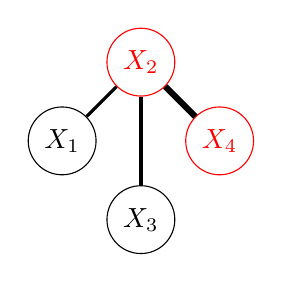
\begin{tikzpicture}
            \node[circle, draw] (A) at (0,0) {$X_1$};
            \node[circle, color=red, draw] (B) at (1,1) {$X_2$};
            \node[circle, draw] (C) at (1,-1) {$X_3$};
            \node[circle, color=red, draw] (D) at (2,0) {$X_4$};
            \draw[line width=0.4mm] (A) -- (B);
            %\draw[line width=0.1mm] (A) -- (C);
            \draw[line width=0.8mm] (B) -- (D);
            \draw[line width=0.5mm] (C) -- (B);
        \end{tikzpicture}
    \end{column}
    \end{columns}

\end{frame}




\begin{frame}{
    General Framework\footnote{See \cite{ektefaie_multimodal_2023,xu_how_2019}}
    }
    General structure: 
    \begin{algorithmic}[1]
    \State Initialize $\nrepresent^{(0)} \gets x_\node, \forall \node \in \NodeSet$ 
        \For{$\iter = 0, ..., \Iter$}:
            \For{$\node \in \Graph$}:
            \State $\nrepresent_{agg}^{\iter+1} \gets \text{Aggregate}(\{h_u^{(\iter)} \mid u \in \nhood_\node\})$
            \State $\nrepresent^{(\iter+1)} \gets \text{Update}(\nrepresent^{(\iter)}, \nrepresent_{agg}^{(\iter)})$
            \EndFor
        \EndFor
        \State $h_\Graph \gets \text{Readout}(h^\Iter_\node | \node \in \Graph)$
    \end{algorithmic}
\vspace{2mm}
Can succinctly represent the $\iter$th layer as: 
\begin{gather*}
    \mathbf{h}_\node^{(\iter+1)} 
    =
    \text{Update}
    \left( 
    x_\node^{(\iter)}
    ,   
    \text{Aggregate}
    (
        h_\node^{(\iter)}, x_u^{(\iter)}, \edge_{u,\node}^{(\iter)}
    )
    \right)
\end{gather*}
\vspace{2mm}
Choices of (differentiable) functions for Aggregate, Update, and Readout determine the architecture of your GNN 
\end{frame}


\begin{frame}{Aggregate/Update}
    \begin{itemize}
        \color{red}
        \item Mention specific functions used 
        \item Mention conequences on architecture/very high level what these steps do wrt graphical structure  
    \end{itemize}
\end{frame}

\begin{frame}{Readout}
    \begin{itemize}
        \color{red}
        \item Permutation invariant function 
        \item Simple function vs pooling
    \end{itemize}
\end{frame}


\begin{frame}{Message Passing}
\end{frame}

\begin{frame}{Graph Convolutional Network}
    Proposed in 2017 by Thomas Kipf, Max Welling \cite{kipf_semi-supervised_2017}
        \begin{align*}
        \iffalse
            \mathbf{h}_\node^{(\iter+1)} 
            &=
            \text{Update}
            \left( 
            x_\node^{(\iter)}
            ,   
            \text{Aggregate}
            (
                h_\node^{(\iter)}, x_u^{(\iter)}, \edge_{u,\node}^{(\iter)}
            )
            \right)
        \\
        \fi 
            \mathbf{H}^{(\iter+1)} 
            &=
            \sigma
            \left( 
                \mathbf{
                %D^{-1/2}
                %(\AdjMat + I)
                %D^{-1/2}
                \Omega 
                H^{(\iter)}
                \Theta 
                }            
            \right)
    \end{align*}
    
    \begin{itemize}
        \item $\mathbf{H}$ is simply the matrix of $\mathbf{h}_\node$ for all nodes 
        \item $\sigma(\cdot) = \text{ReLu}(\cdot)$ activation function
        \item Learned weight/parameter matrix $\boldsymbol\Theta$
        \item Including $\boldsymbol\Omega$ normalizing matrix (with known closed form) for computational stability, function of $\AdjMat$ or $\LapMat$
        %\item $\mathbf{D}_{ii} = \sum_{j}\mathbf{(\AdjMat+I)_{ij}}$
        %\item Eigenvalue normalizing $\mathbf{D^{-1/2}(\AdjMat + I)D^{-1/2}}$ for computational stability
    \end{itemize}
    \textcolor{red}{Review paper, comment on applications briefly (KG setting)}
    \end{frame}



\section{Applications and Extensions \textcolor{red}{20-25ish minutes}}
\OutlineRedux


\subsection{Knowledge-Graph Data}

\subsection{Multimodal Biomedical Data}




\begin{frame}{}
    \bf{\LARGE Conclusion}    
\end{frame}

\section*{Conclusion}



\begin{frame}[allowframebreaks]{References}
    \begin{itemize}
    \item Some diagrams generated in conjunction with ChatGPT 3.5
    \end{itemize}
    \printbibliography 
\end{frame}


%%%%%%%%%%%%%%%%%%%%%%%%%%
%%%%%%%%%%%%%%%%%%%%%%%%%%
% Appendix 
%%%%%%%%%%%%%%%%%%%%%%%%%%
%%%%%%%%%%%%%%%%%%%%%%%%%%

\section*{Appendix}

\begin{frame}{}
\bf{\LARGE Appendix Slides}    
\end{frame}

\begin{frame}{Abbreviated History}
    \begin{itemize}
        \item Graph Neural Network first used in Scarselli (2009) {\it The Graph Neural Network Model} \cite{scarselli_graph_2009}
        \item Graph Convolutional Network by Kipf (2017) \cite{kipf_semi-supervised_2017} but with similar convolutional message-passing algorithms proposed in 2015 \cite{duvenaud_convolutional_2015}
        \item Message passing GNN proposed in Gilmer (2017), applications in molecular chemistry \cite{gilmer_neural_2017} 
    \end{itemize}
\end{frame}

\begin{frame}{}
    Full figure from McDermott et al. \cite{mcdermott_structure-inducing_2023}, cropped and presented in Introduction:
    \begin{figure}
        \centering
        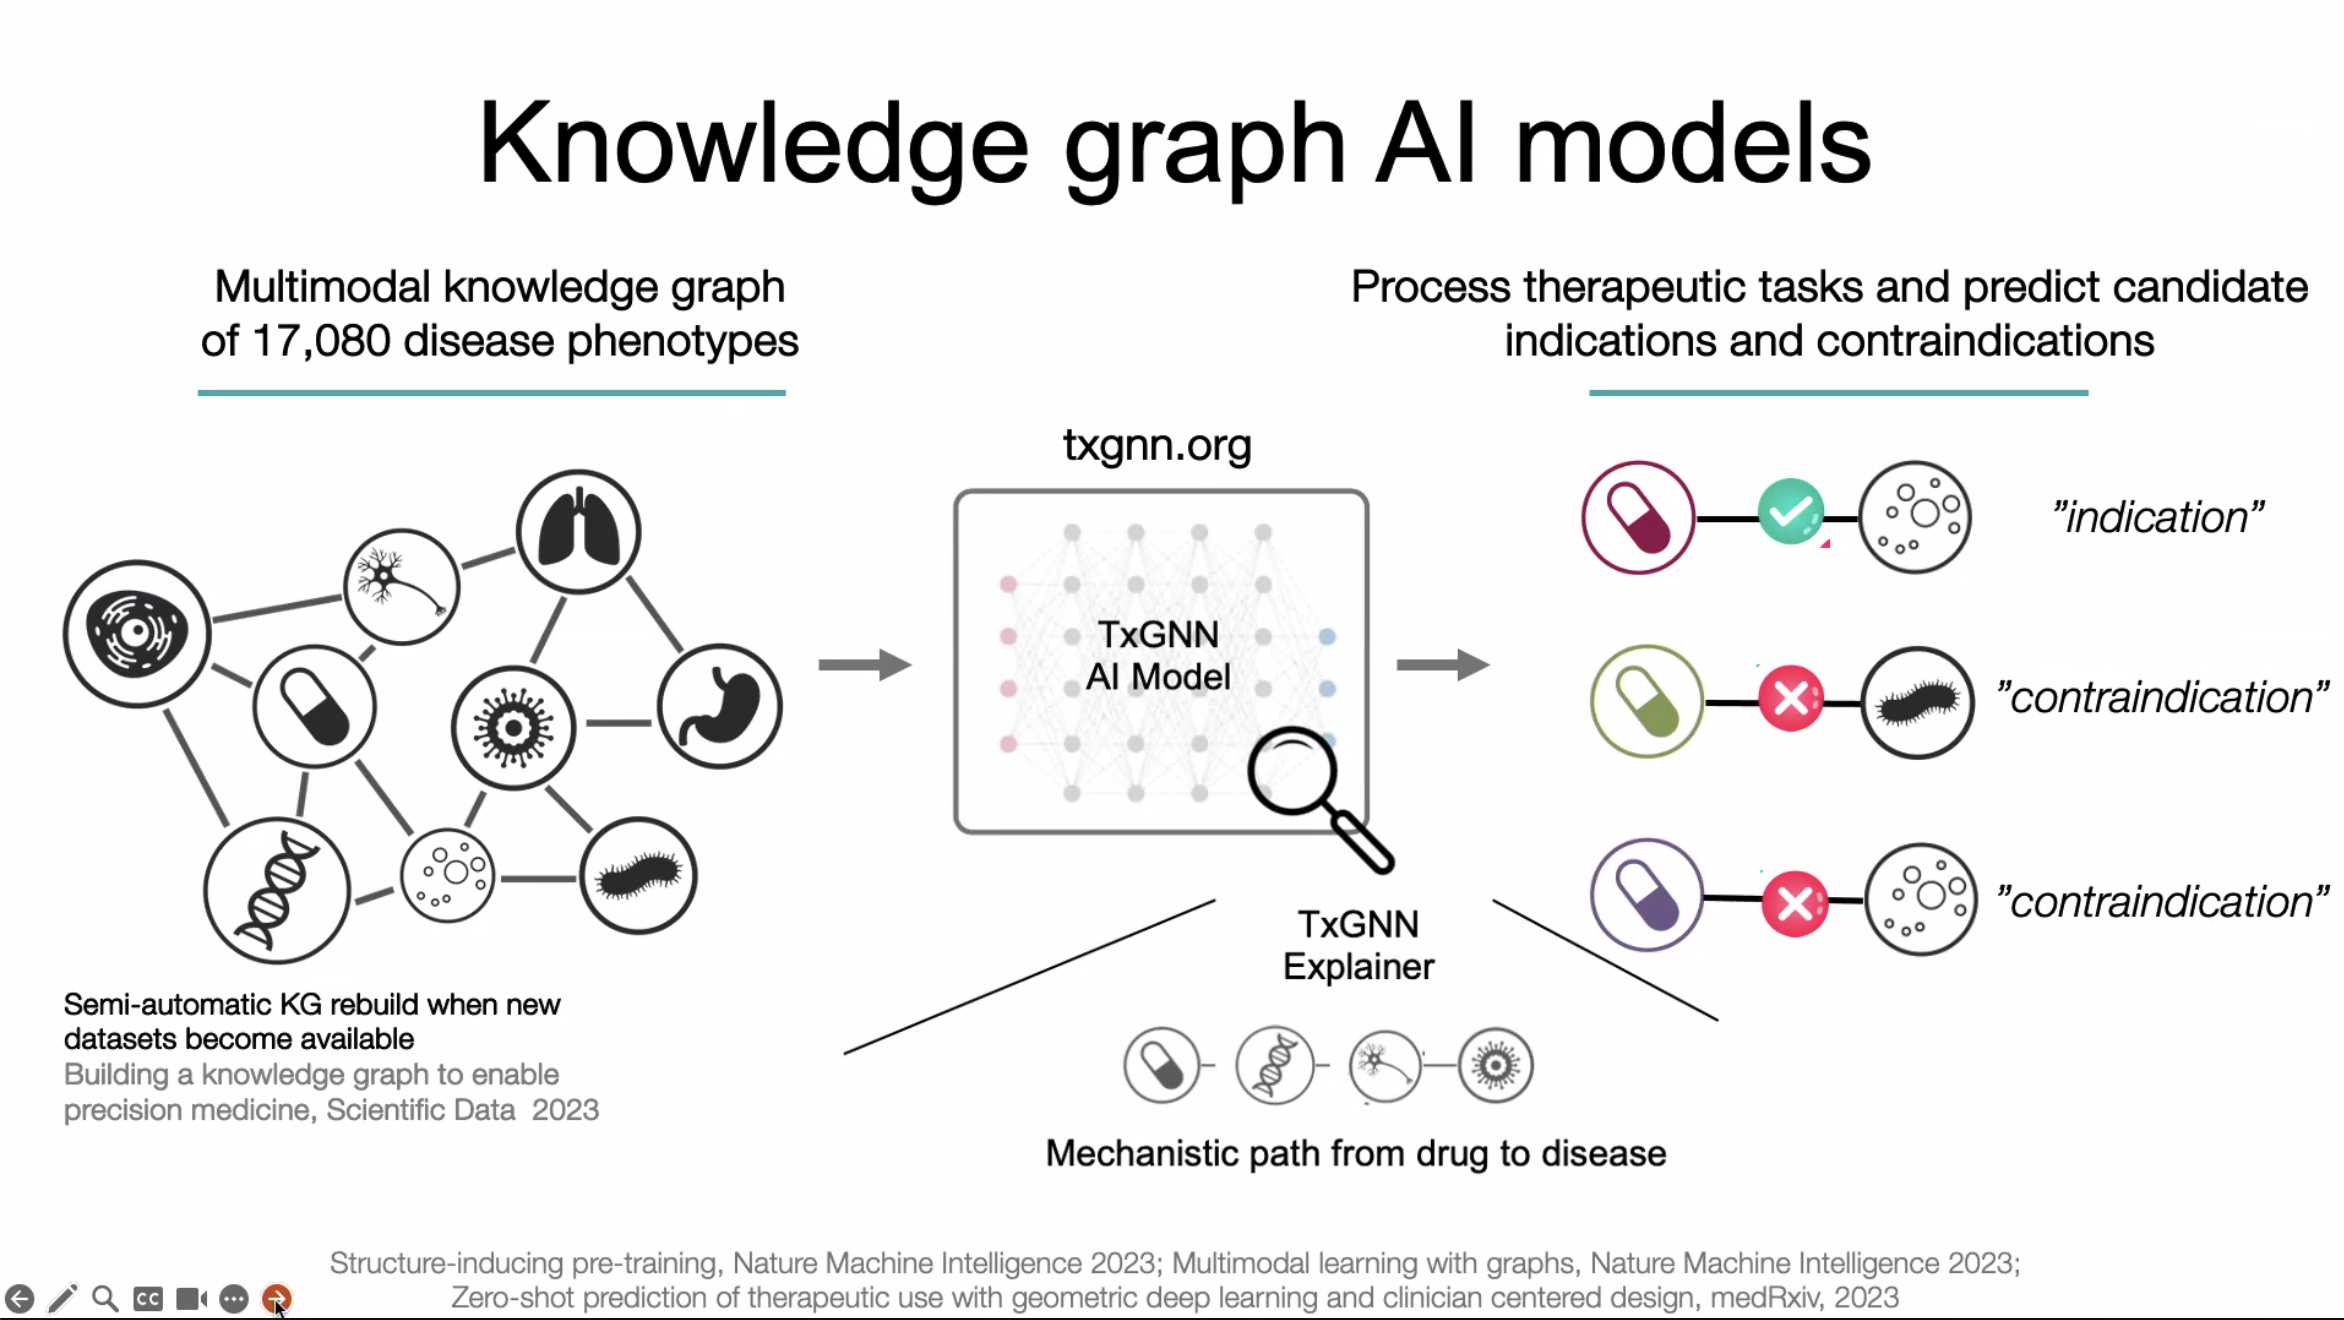
\includegraphics[scale=0.13]{Junwei_KG_Models_Infograph.png}
    \end{figure}
\end{frame}
\end{document}